% Section 8: the teamwork record and the meeting evidence.
% The assignment asks for evidence of at least two team meetings.
% Paste the meeting screenshots over the two TODO markers below.
% The example figure block stays commented out until a picture file exists.

\section{Meetings}

We couldn't arrange an in-person meeting so both meetings are held online as listed in Table~\ref{tab:meetings}.

\begin{table}[tb]
  \centering
  \footnotesize
  \setlength{\tabcolsep}{4pt}
  \begin{tabular}{@{}c p{0.11\textwidth} p{0.15\textwidth}
                    p{0.20\textwidth} p{0.36\textwidth}@{}}
    \toprule
    No. & Date & Mode & Attendees & Decisions \\
    \midrule
    1 & \textbf{3.10.2026} & \textbf{Online}
    & \textbf{Yusuf, Erdem, Mehmet}
    & \textbf{Yusuf, Erdem and Mehmet works on GAN, Autoencoder and Diffusion respectively.} \\
    2 & \textbf{10.10.2026} & \textbf{Online}
    & \textbf{Yusuf, Erdem, Mehmet and Eren}
    & \textbf{Discussion of findings and division of tasks for report and presentation creation.} \\
    \bottomrule
  \end{tabular}
  \caption{The team meetings.}
  \label{tab:meetings}
\end{table}

\begin{center}
  \fbox{\parbox{0.92\textwidth}{\centering \textbf{
    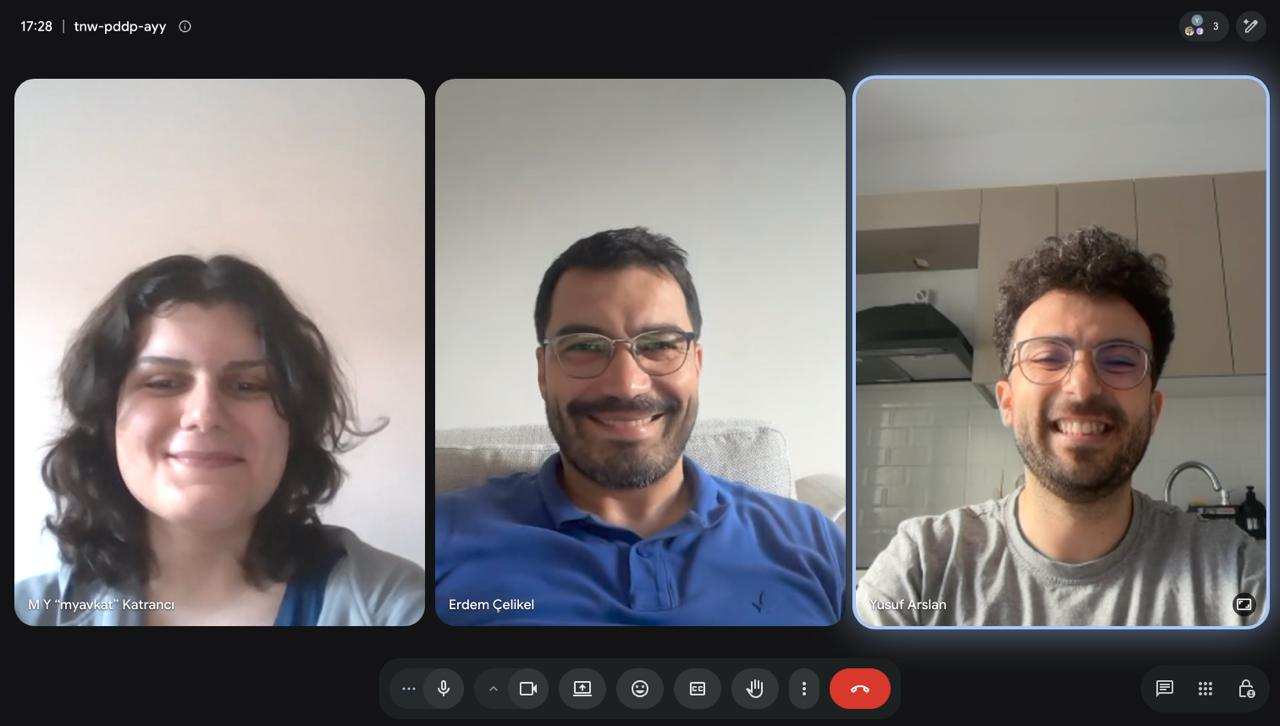
\includegraphics[width=0.85\textwidth]{figures/Toplanti1.jpeg}
    \captionof{figure}{The first team meeting.}
    \label{fig:meeting1}
  }}}
\end{center}

\medskip

\begin{center}
  \fbox{\parbox{0.92\textwidth}{\centering \textbf{
    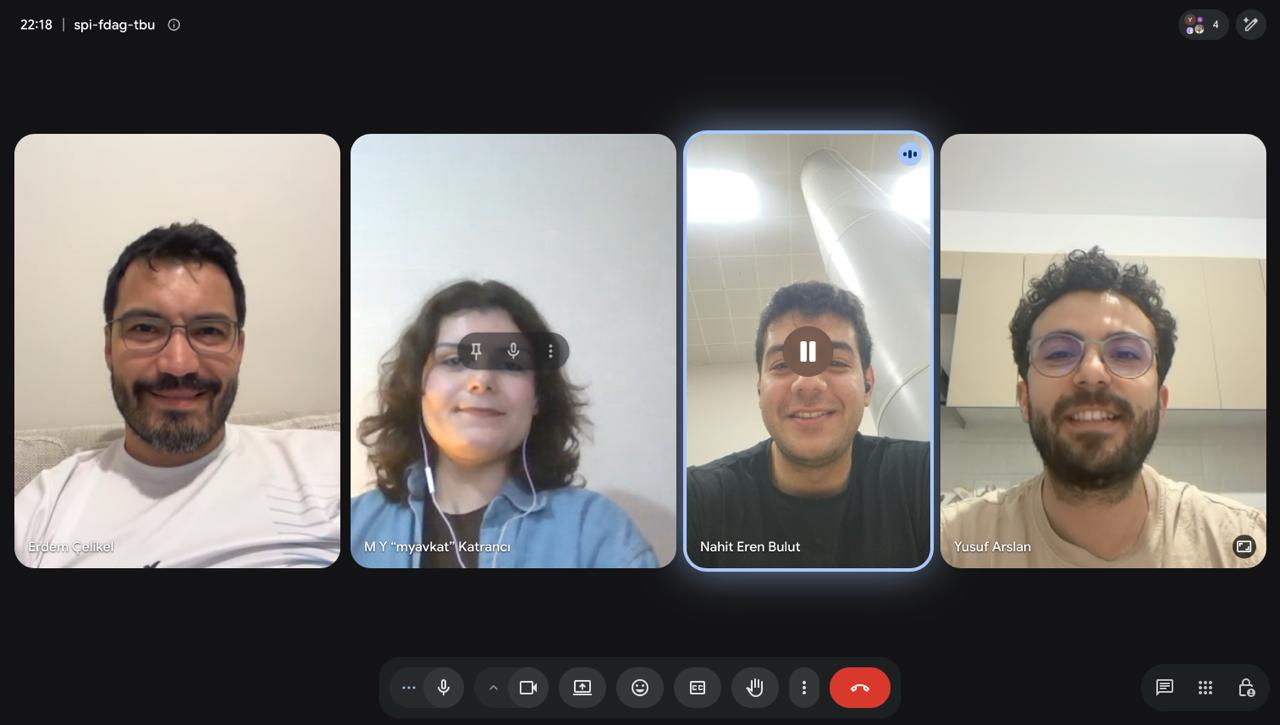
\includegraphics[width=0.85\textwidth]{figures/Toplanti2.jpeg}
    \captionof{figure}{The second team meeting.}
    \label{fig:meeting2}
  }}}
\end{center}

% When a picture is ready, uncomment and adjust this example block:
% \begin{figure}[tb]
%   \centering
%   \includegraphics[width=0.85\textwidth]{figures/meeting_1.png}
%   \caption{The first team meeting.}
%   \label{fig:meeting1}
% \end{figure}

The team divided the work by method, and each member wrote the part of the
report that covers that method. \textbf{Erdem} built and trained
the autoencoder, \textbf{Yusuf} ran the FOMM experiment,
\textbf{Mehmet} ran the rectified flow pipeline, and
\textbf{Eren} wrote the shared chapters and the slides.
